
\section{Análisis univariado (variables cuantitativas)}
\label{sec:variablescuantitativas} 
\subsubsection{Recency}
\begin{figure}[H]
\centering
\begin{subfigure}[b]{0.47\textwidth}
    \centering
    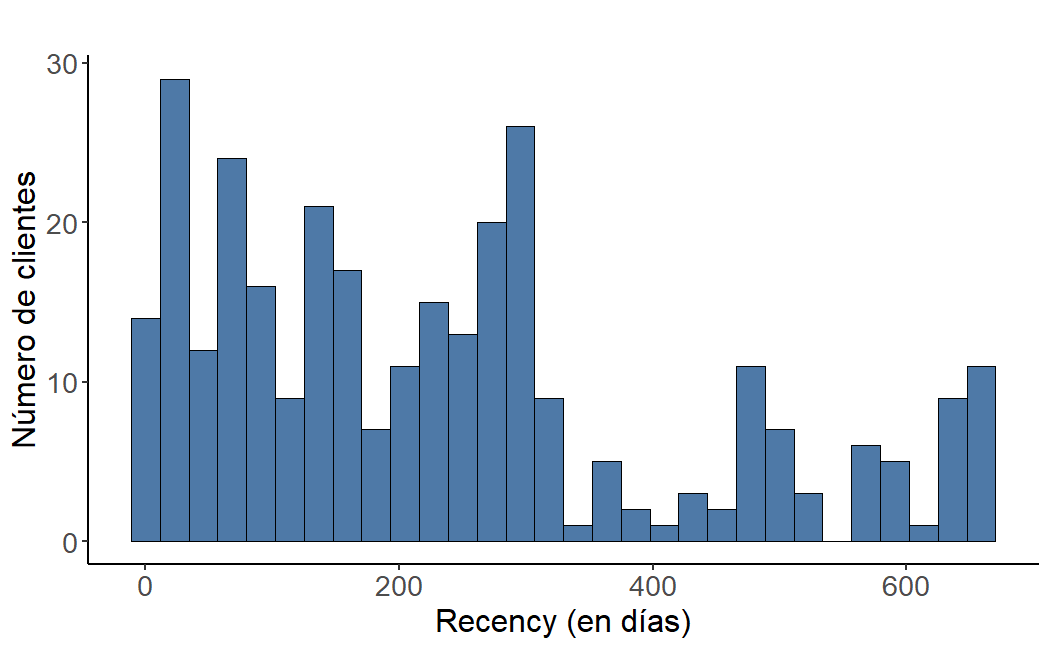
\includegraphics[width=\textwidth]{figuras/Recency.png}
    \caption{Histograma}
    \label{fig:recency_histograma}
\end{subfigure}
\hspace{0.01\textwidth} 
\begin{subfigure}[b]{0.47\textwidth}
    \centering
    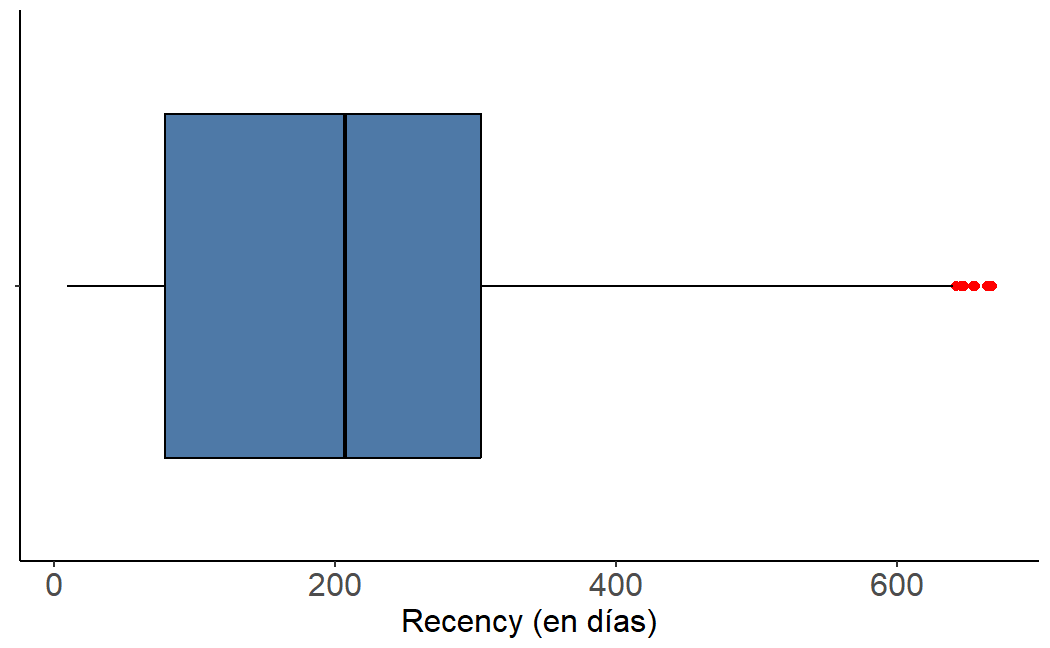
\includegraphics[width=\textwidth]{figuras/Boxplot Recency.png}
    \caption{Boxplot}
    \label{fig:boxplot_recency}
\end{subfigure}
\caption{Distribución de recency}
\label{fig:recency_boxplot_hist}
\end{figure}
\subsubsection{Frequency}
\begin{figure}[H]
\centering
\begin{subfigure}[b]{0.47\textwidth}
    \centering
    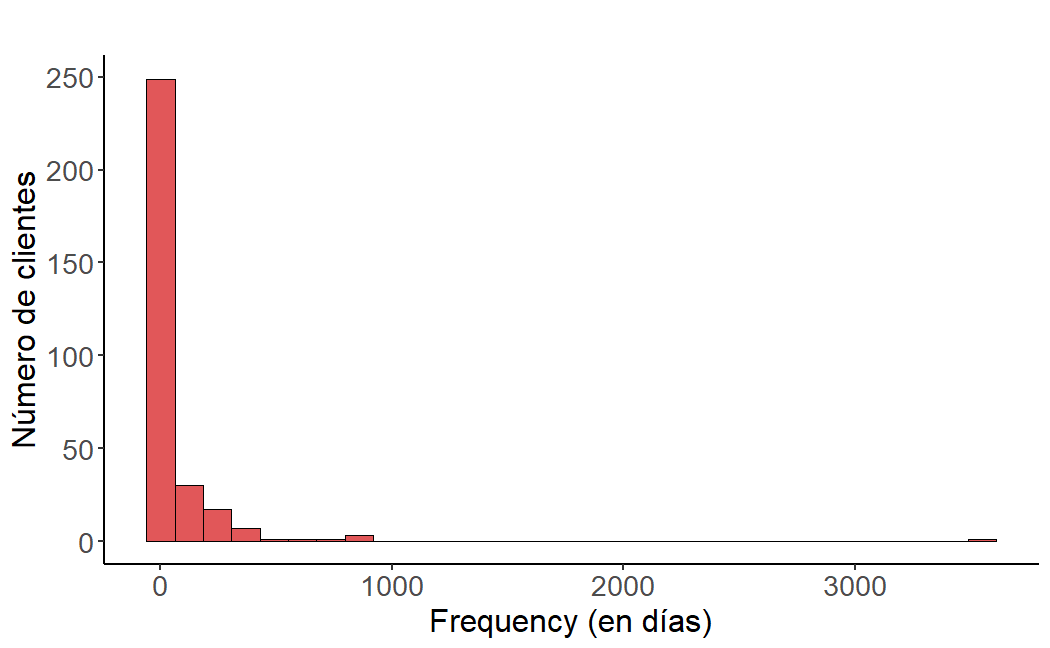
\includegraphics[width=\textwidth]{figuras/Frequency.png}
    \caption{Histograma}
    \label{fig:frequency_histograma}
\end{subfigure}
\hspace{0.01\textwidth}
\begin{subfigure}[b]{0.47\textwidth}
    \centering
    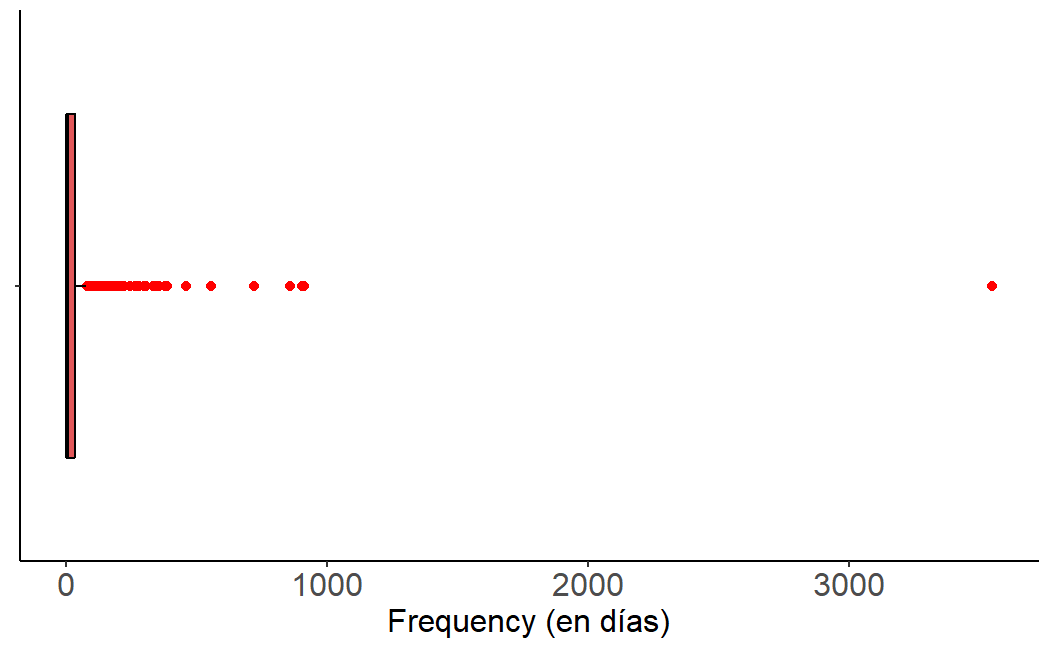
\includegraphics[width=\textwidth]{figuras/Boxplot_Frequency.png}
    \caption{Boxplot}
    \label{fig:frequency_boxplot}
\end{subfigure}
\caption{Distribución de frequency}
\label{fig:recency_boxplot}
\end{figure}

\subsubsection{Monetary}
\begin{figure}[H]
\centering
\begin{subfigure}[b]{0.47\textwidth}
    \centering
    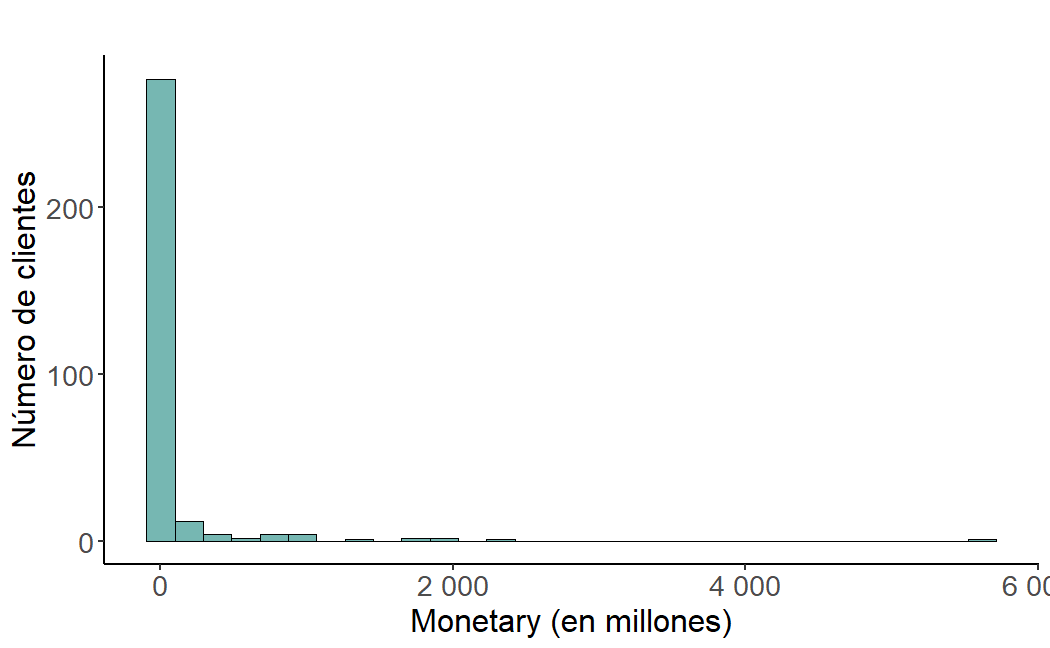
\includegraphics[width=\textwidth]{figuras/Monetary.png}
    \caption{Histograma}
    \label{fig:Histograma_Monetary}
\end{subfigure}
\hspace{0.01\textwidth}
\begin{subfigure}[b]{0.47\textwidth}
    \centering
    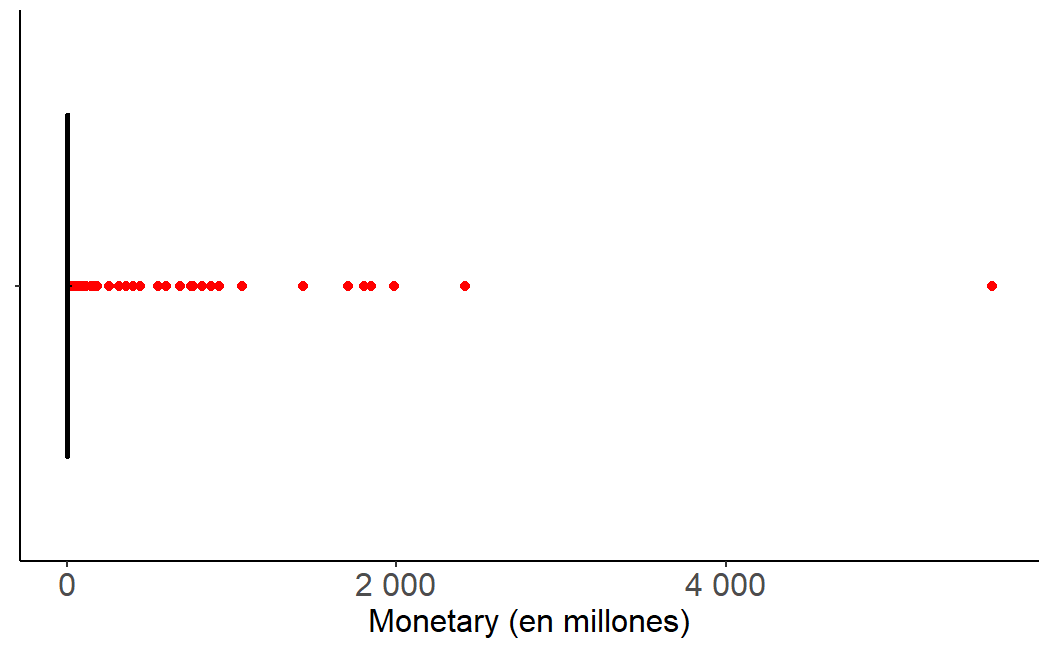
\includegraphics[width=\textwidth]{figuras/Boplot_Monetary.png}
    \caption{Boxplot}
    \label{fig:boxplotmonetary}
\end{subfigure}
\caption{Distribución de monetary}
\label{fig:monetary}
\end{figure}

\subsubsection{Valor Neto}
\begin{figure}[H]
\centering
\begin{subfigure}[b]{0.47\textwidth}
    \centering
    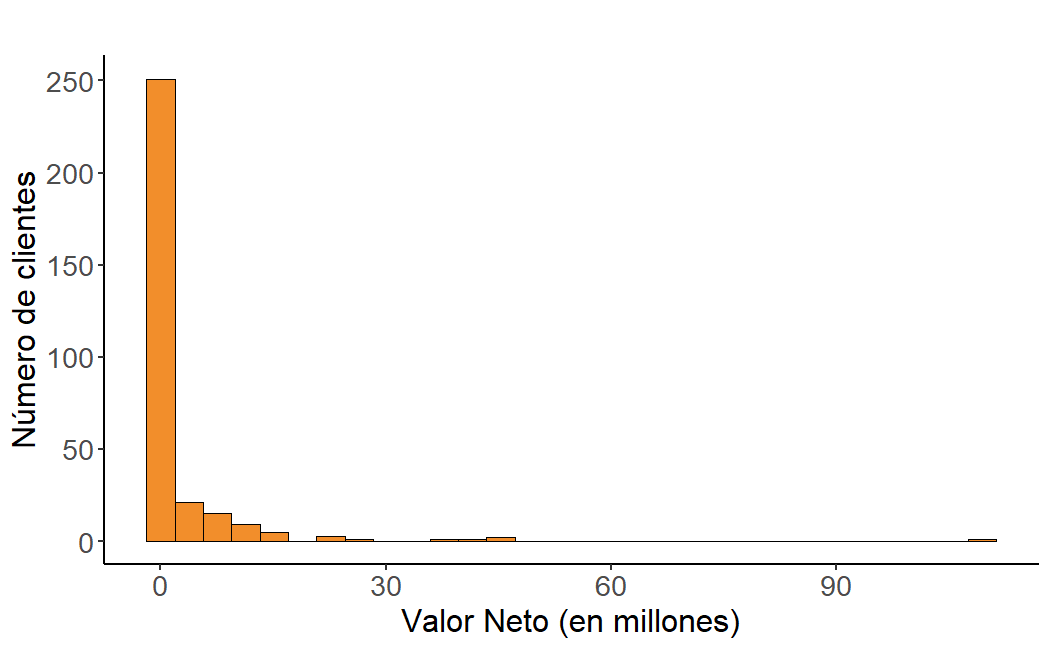
\includegraphics[width=\textwidth]{figuras/Valor Neto.png}
    \caption{Histograma }
    \label{fig:Histograma_Valor Neto}
\end{subfigure}
\hspace{0.01\textwidth}
\begin{subfigure}[b]{0.47\textwidth}
    \centering
    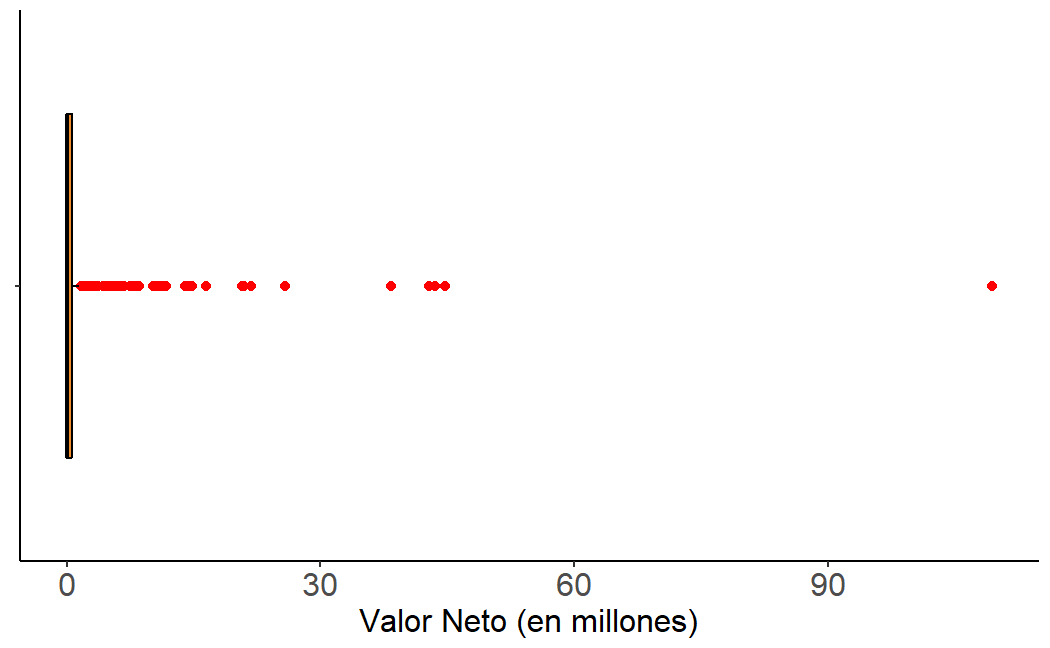
\includegraphics[width=\textwidth]{figuras/Boxplot Valor Neto.png}
    \caption{Boxplot}
    \label{fig:boxplotvalorneto}
\end{subfigure}
\caption{Distribución de la variable valor neto}
\label{fig:valor neto}
\end{figure}

\subsubsection{Valor Bruto}
\begin{figure}[H]
\centering
\begin{subfigure}[b]{0.47\textwidth}
    \centering
    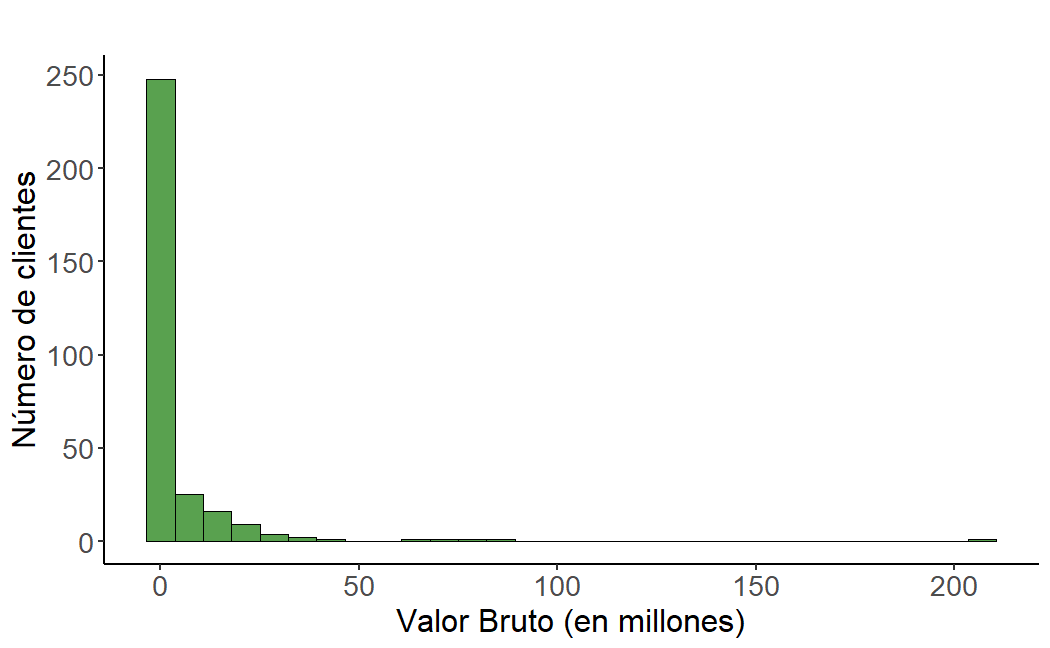
\includegraphics[width=\textwidth]{figuras/Histograma Valor Bruto.png}
    \caption{Histograma}
    \label{fig:Histograma_Valor Bruto}
\end{subfigure}
\hspace{0.01\textwidth}
\begin{subfigure}[b]{0.47\textwidth}
    \centering
    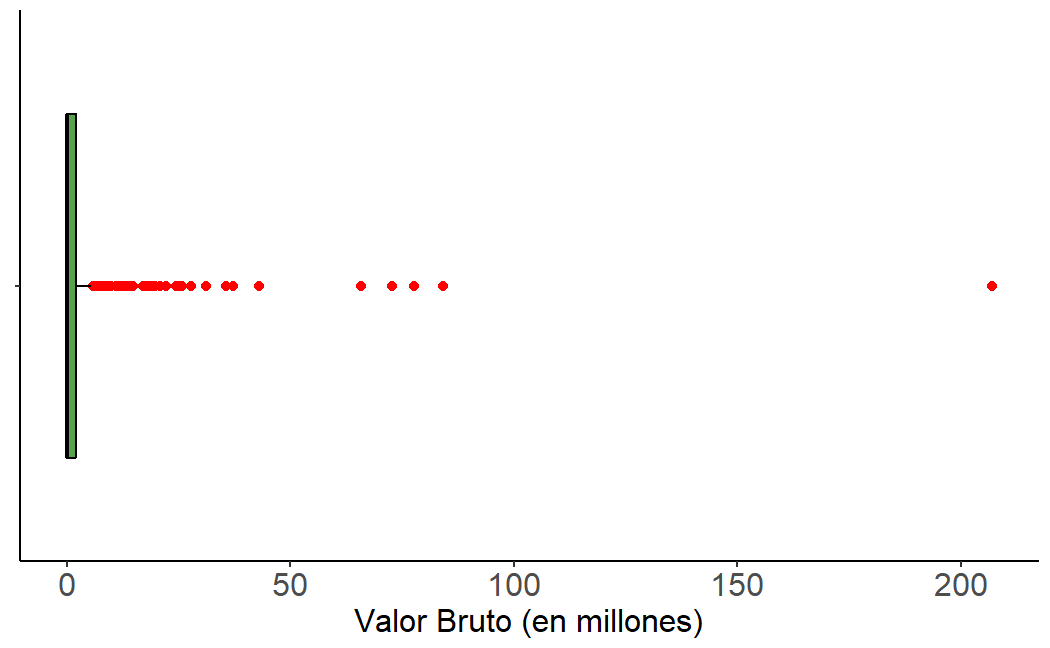
\includegraphics[width=\textwidth]{figuras/Boxplot Valor Bruto.png}
    \caption{Boxplot}
    \label{fig:boxplotvalorbruto}
\end{subfigure}
\caption{Distribución del valor bruto}
\label{fig:valor bruto}
\end{figure}

\subsubsection{Costo Total}
\begin{figure}[H]
\centering
\begin{subfigure}[b]{0.47\textwidth}
    \centering
    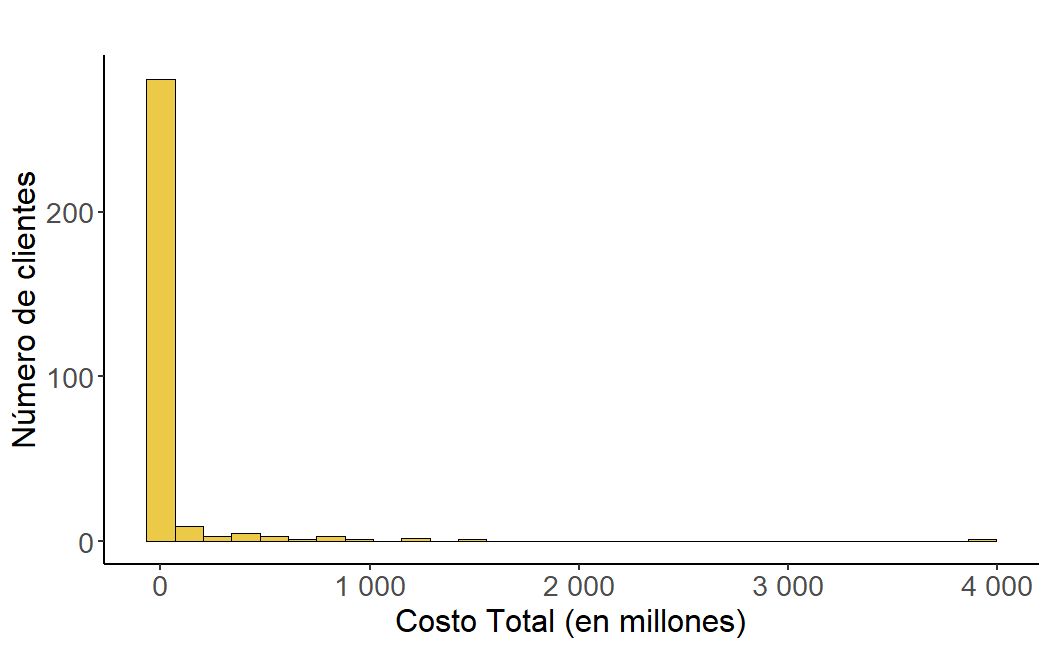
\includegraphics[width=\textwidth]{figuras/Histograma - Costo Total.png}
    \caption{Histograma}
    \label{fig:Histograma_Costo Total}
\end{subfigure}
\hspace{0.01\textwidth}
\begin{subfigure}[b]{0.47\textwidth}
    \centering
    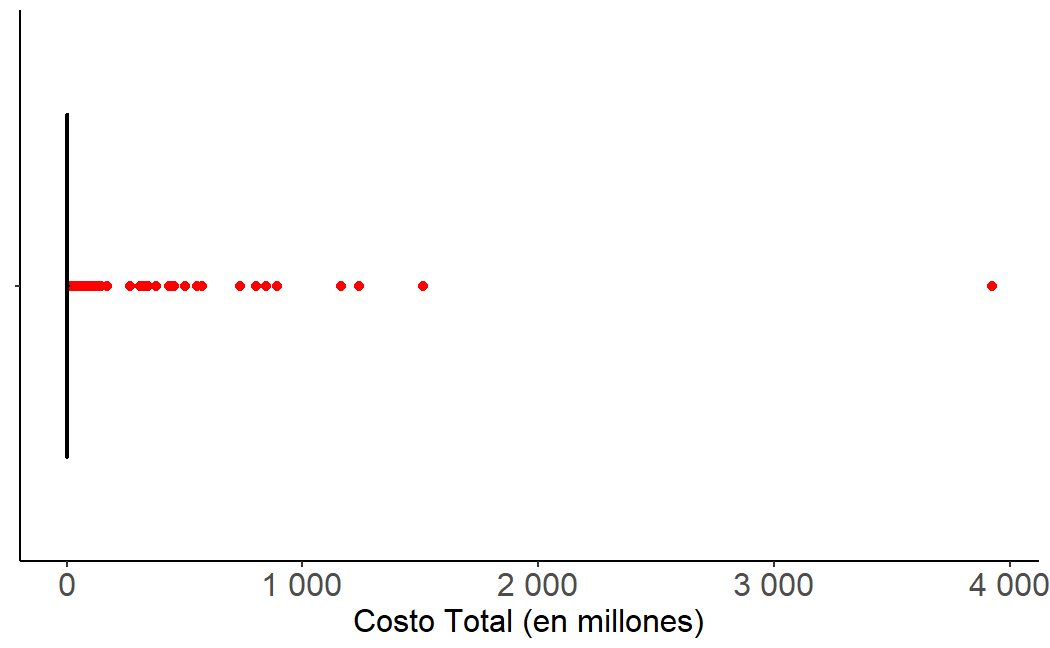
\includegraphics[width=\textwidth]{figuras/Boxplot - Costo Total.png}
    \caption{Boxplot}
    \label{fig:boxplotcostotal}
\end{subfigure}
\caption{Distribución del costo total}
\label{fig:costo total}
\end{figure}

\subsubsection{Cantidad}
\begin{figure}[H]
\centering
\begin{subfigure}[b]{0.47\textwidth}
    \centering
    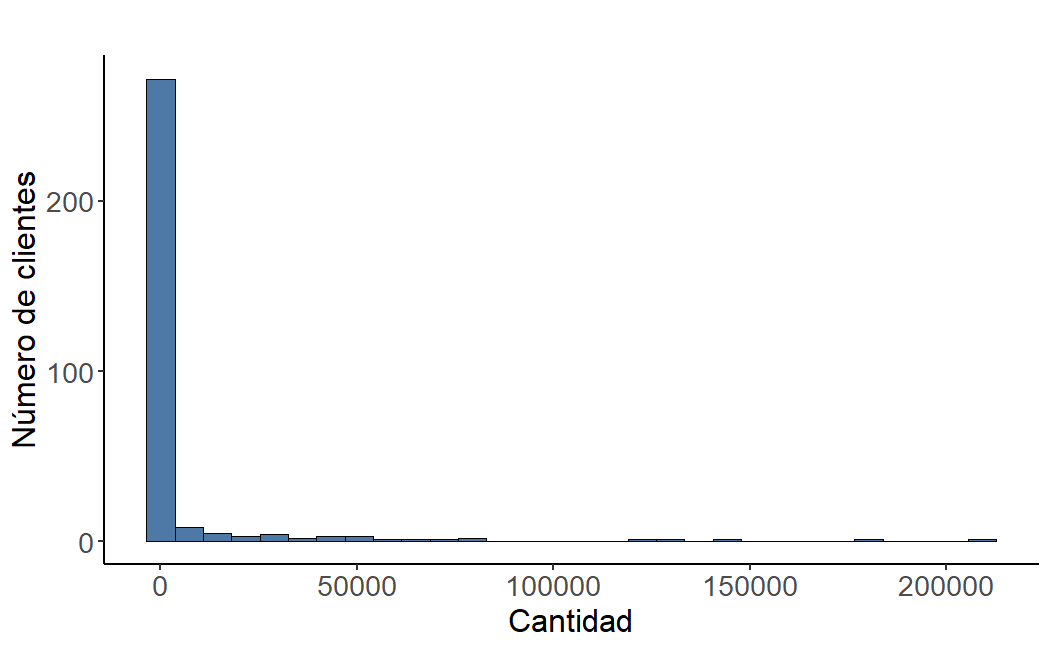
\includegraphics[width=\textwidth]{figuras/Histograma Cantidad.png}
    \caption{Histograma}
    \label{fig:Histograma_Cantidad}
\end{subfigure}
\hspace{0.01\textwidth}
\begin{subfigure}[b]{0.47\textwidth}
    \centering
    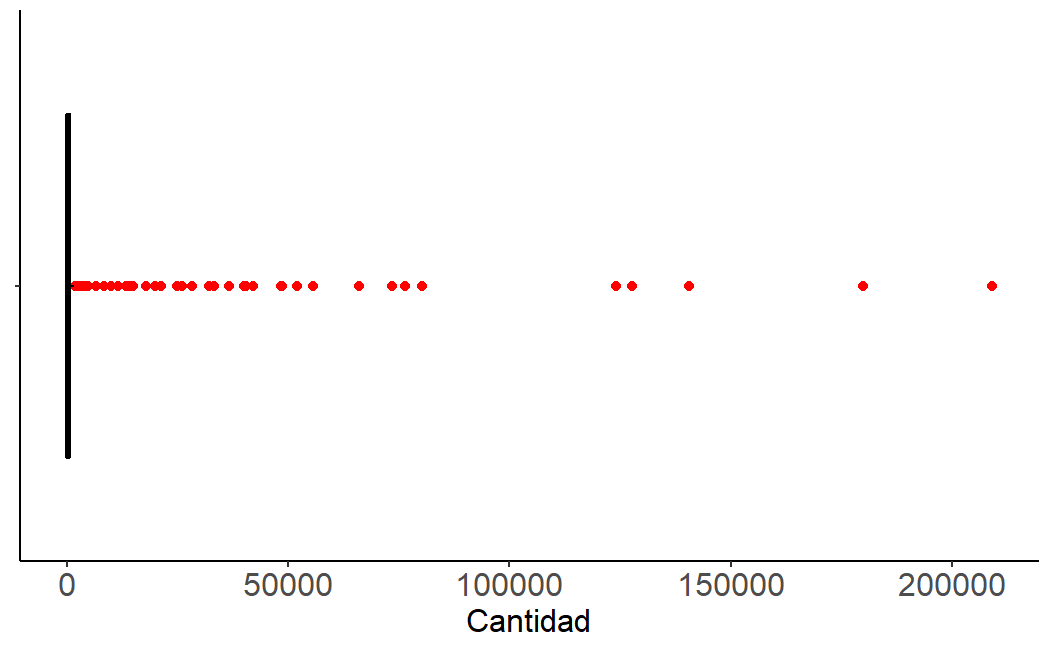
\includegraphics[width=\textwidth]{figuras/Boxplot - Cantidad.png}
    \caption{Boxplot}
    \label{fig:boxplotcantidad}
\end{subfigure}
\caption{Distribución de la variable cantidad}
\label{fig:cantidad}
\end{figure}

\subsubsection{Descuentos}
\label{sec:variablesdescuentos}
\begin{figure}[H]
\centering
\begin{subfigure}[b]{0.47\textwidth}
    \centering
    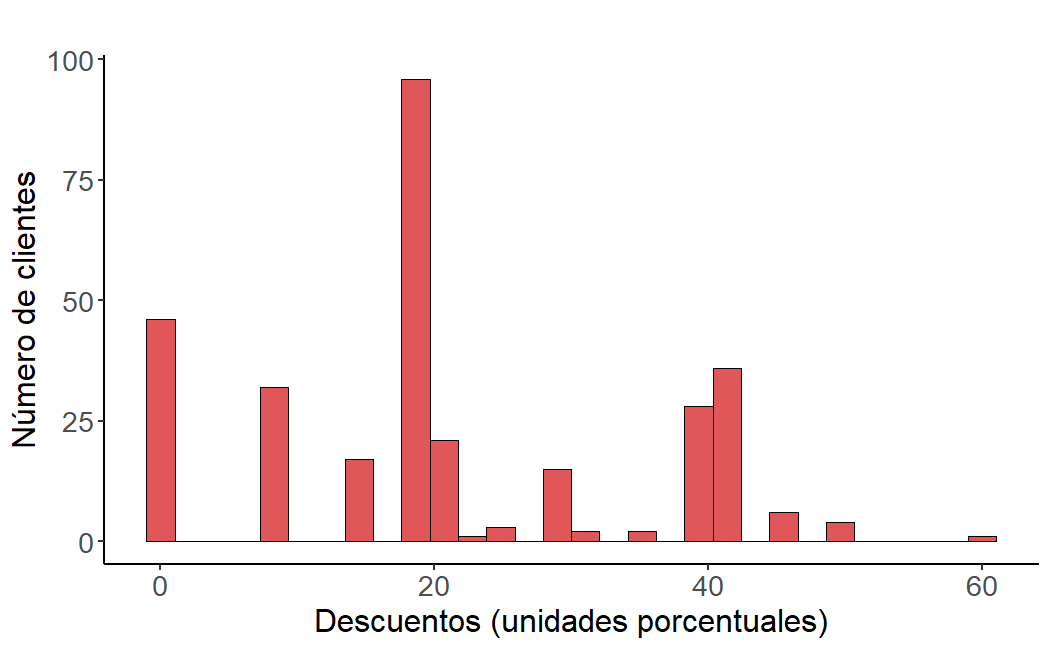
\includegraphics[width=\textwidth]{figuras/Histograma - Descuentos.png}
    \caption{Histograma}
    \label{fig:Histograma_Descuentos}
\end{subfigure}
\hspace{0.01\textwidth}
\begin{subfigure}[b]{0.47\textwidth}
    \centering
    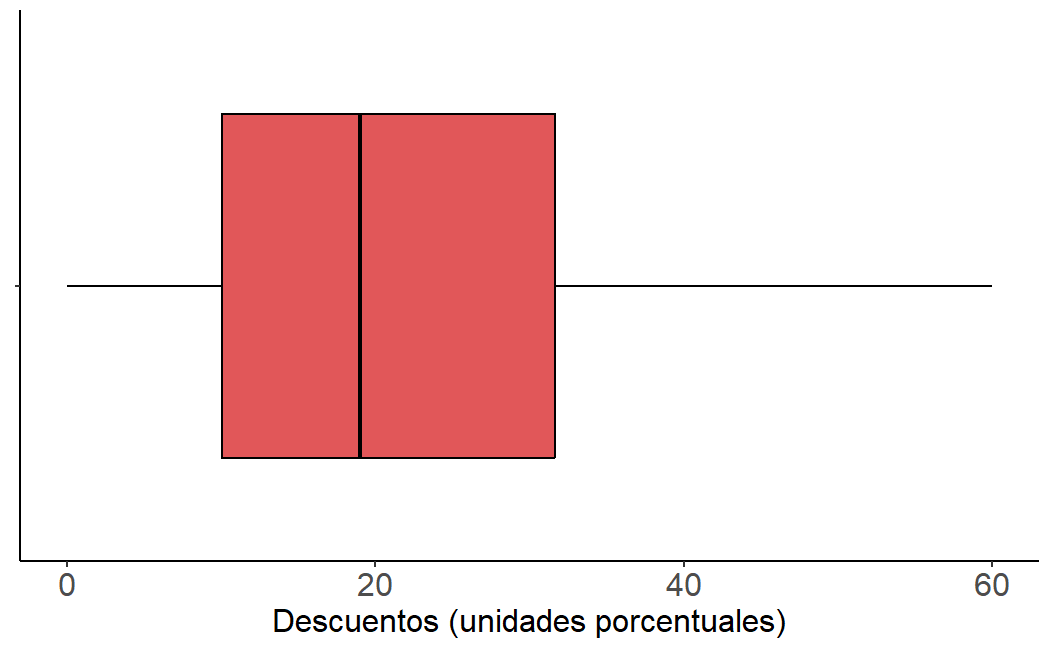
\includegraphics[width=\textwidth]{figuras/Boxplot Descuentos.png}
    \caption{Boxplot}
    \label{fig:boxplotdescuentos}
\end{subfigure}
\caption{Distribución del descuentos}
\label{fig:descuentos}
\end{figure}

\subsubsection{Skus distintos}
\begin{figure}[H]
\centering
\begin{subfigure}[b]{0.47\textwidth}
    \centering
    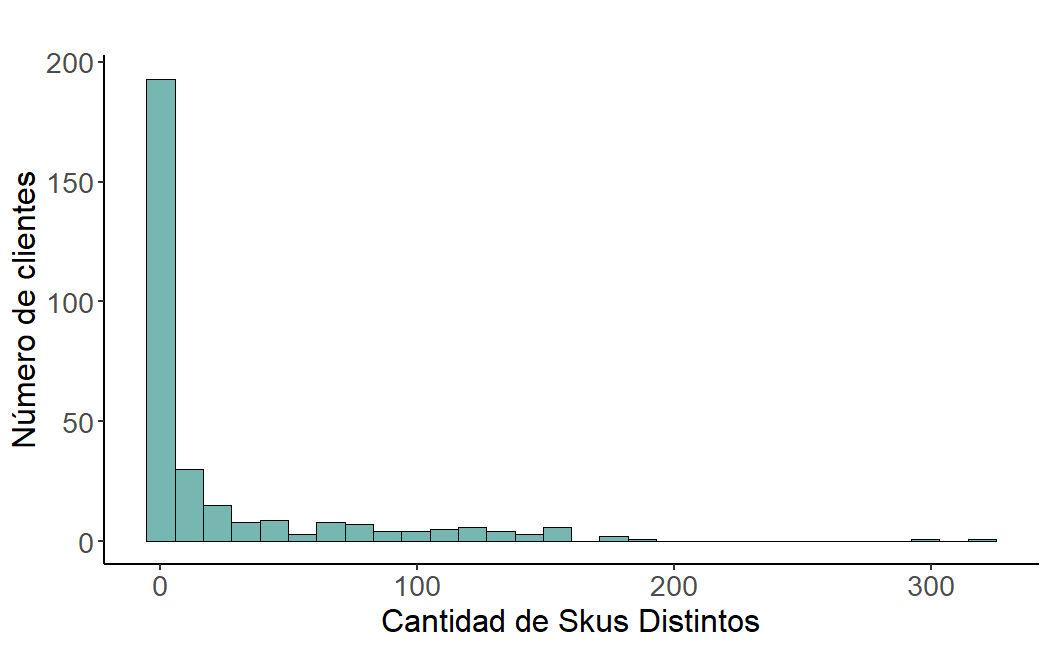
\includegraphics[width=\textwidth]{figuras/Histograma - Skus distintos.png}
    \caption{Histograma}
    \label{fig:Histograma_Skus distintos}
\end{subfigure}
\hspace{0.01\textwidth}
\begin{subfigure}[b]{0.47\textwidth}
    \centering
    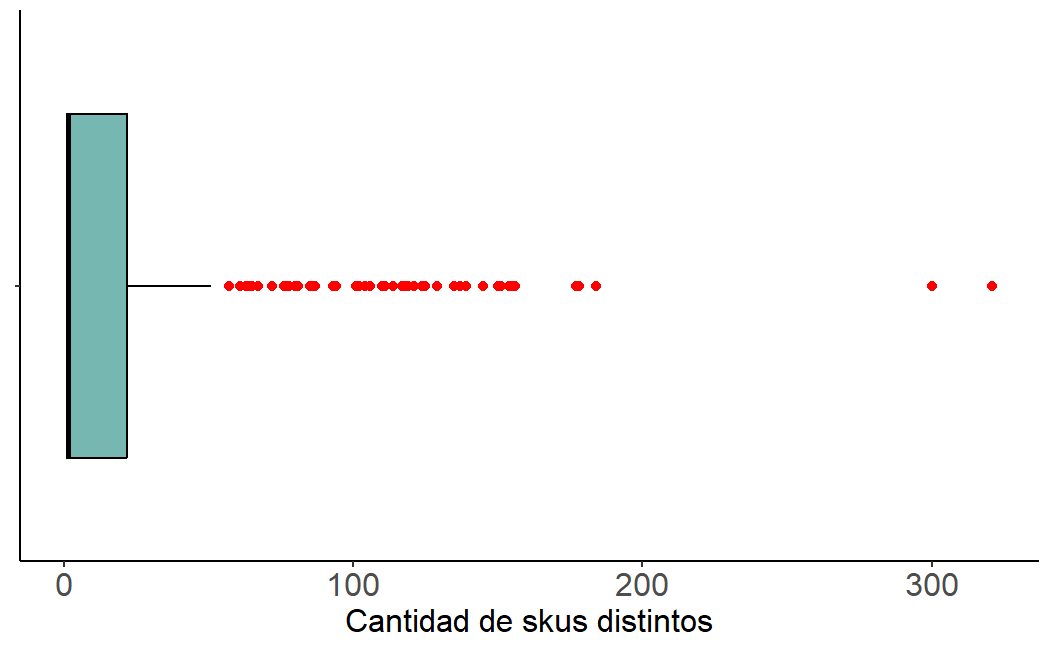
\includegraphics[width=\textwidth]{figuras/Boxplot - Skus Distintos.png}
    \caption{Boxplot}
    \label{fig:boxplotskusdistintos}
\end{subfigure}
\caption{Distribución del número de Skus distintos}
\label{fig:skusdistintos}
\end{figure}
\subsection{Análisis multivariado}
\subsubsection{Matriz de correlación Spearman - variables cuantitativas}
\begin{figure}[H]
\centering
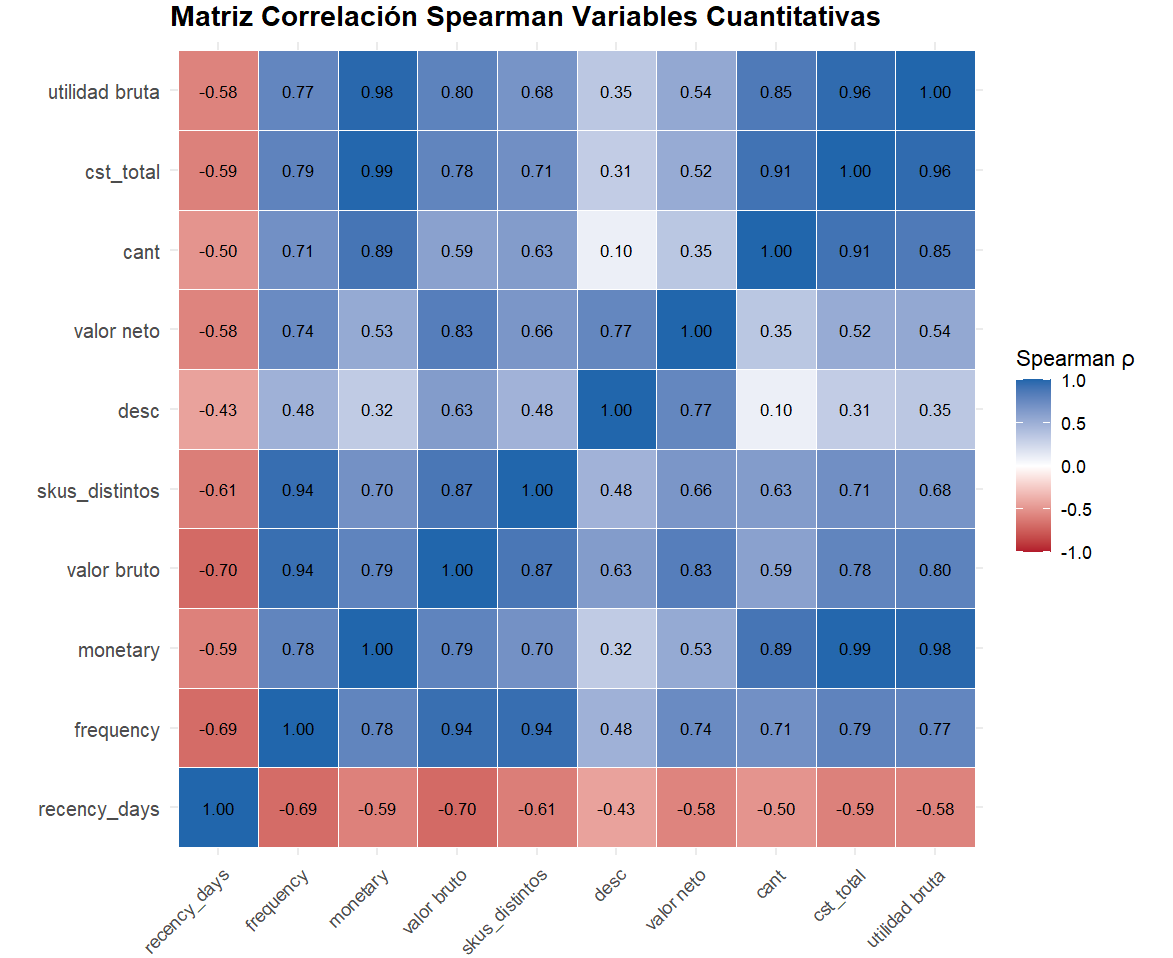
\includegraphics[width=0.8\textwidth]{figuras/CORR_CUANT.png}
\caption{Correlación Spearman Variables Cuantitativas.}
\label{fig:corr_cuantitativas} 
\end{figure}
\subsubsection{Matriz de correlación Cramer - variables cualitativas}
\begin{figure}[H]
\centering
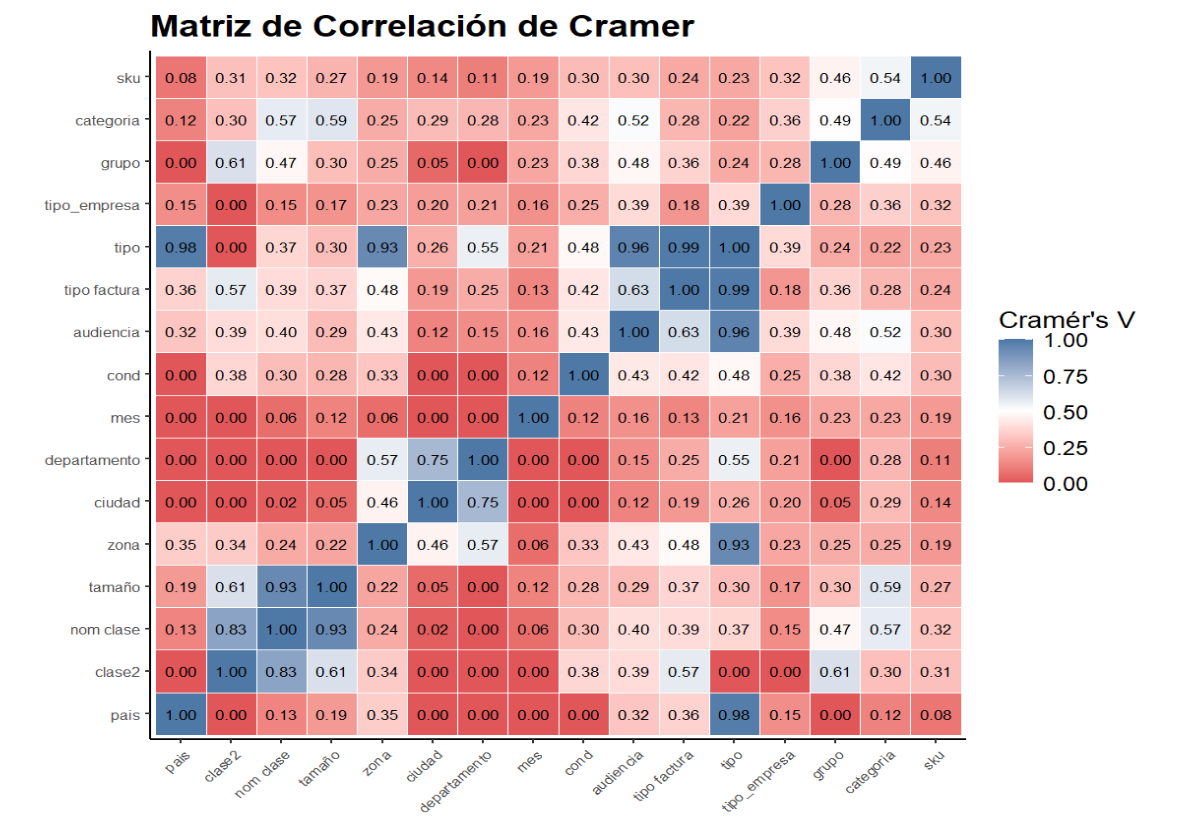
\includegraphics[width=\linewidth]{figuras/Cramer.png} % o \textwidth
\caption{\label{figCramer}Correlación Cramer - variables cualitativas.}
\end{figure}

\clearpage
\printbibliography